\documentclass[11pt,a4paper,titlepage]{report} 
\usepackage[utf8]{inputenc} 
\usepackage[french]{babel} 
\usepackage[T1]{fontenc} 
\usepackage{amsmath} 
\usepackage{amsfonts} 
\usepackage{amssymb} 
\usepackage{graphicx} 
\usepackage[final]{pdfpages} 
\usepackage[toc,page]{appendix} 
\usepackage[top=2.5cm,bottom=2.5cm,right=2.5cm,left=2.5cm]{geometry} 

\newcommand{\HRule}{\rule{\linewidth}{0.5mm}}

\begin{document}

\begin{titlepage}
\begin{center}

% Upper part of the page. The '~' is needed because \\
% only works if a paragraph has started.
%
\includegraphics[width=0.15\textwidth]{./logo}~\\[1cm]

\includegraphics[width=0.15\textwidth]{logo.png}~
\\[1cm]
\textsc{\LARGE iut informatique de belfort-montbéliard}\\[1cm]

\textsc{\Large Projet de base de données}\\[0.5cm]

% Title
\HRule \\[0.4cm]
{ \huge \bfseries Velacampus website \\[0.4cm] }

\HRule \\[1.5cm]

% Author and supervisor
\begin{minipage}{0.4\textwidth}
\begin{flushleft} \large
\emph{Auteur:}\\
Morgane \textsc{cabrol}\\
Pierre \textsc{limballe}\\
Geoffrey \textsc{glangine}\\
Auguste \textsc{meyer}
\end{flushleft}
\end{minipage}
\begin{minipage}{0.4\textwidth}
\begin{flushright} \large
\emph{Superviseur:} \\
Alexandru  \textsc{dobrila}
\end{flushright}
\end{minipage}

\vfill

% Bottom of the page
{\large \today}

\end{center}
\end{titlepage}

\tableofcontents
\chapter*{Introduction}
introduction...
\chapter{Le cahier des charges}
Partie admistrateur :  
La partie adnistrateur est accéssible par deux admins et certaines parties sont accéssible par des modos aussi    
 Mail liste des adhérents  
(nom, prénom, formation, date de naissance, lieu de naissance, adresse, code postale, téléphone portable, adresse e-mail, photos)
  Suivi des vélos  
(numéro vélo, numeros cadenas(3 cadenas), date location, état du vélo, durée location, prolongation (ou non), date retour, état de retour)
  Demande de cotisation + acceptation de la demande
(photos ou paiement en attente)
  Chat-box entre admin et modo
  Ra-jout de fiche vélo, fiche de suivi 
 Modification des fiches vélos, fiches de suivi
  Suivi de réparation du vélo  
(type réparation, pièce changée, cout réparation, date réparation)
  Ajout de photos/informations
  Importation d'un calendrier google+
 Administration du forum
  Archive en PDF
(Archive de vélocampus, compte rendu de réunion ect ...)


Partie publique
Certaines parties ne sont accéssible que par les adhérents connectés 
 Formulaire d'adhésion
 Formulaire de demande de réparation  
(disponibilité du demandeur, urgence ou non de la réparation, type de problème, numero vélo, numero adhérents)
 Formulaire de demande de location  
(que pour les adhérents (donc personne connecté au site), Etat réservation (validé, en attente, refusé))
  Calendrier en ligne avec les évenements
  page présentation, page équipe, page photos, page projet ...
  Forum avec possibilité d'ajouter des sujets
  Compte pour les adhérents  
(avec identifiants, mot de passe et photos)

\chapter{Base de données}
\section{le modèle conceptuel de donnée}
\begin{center}
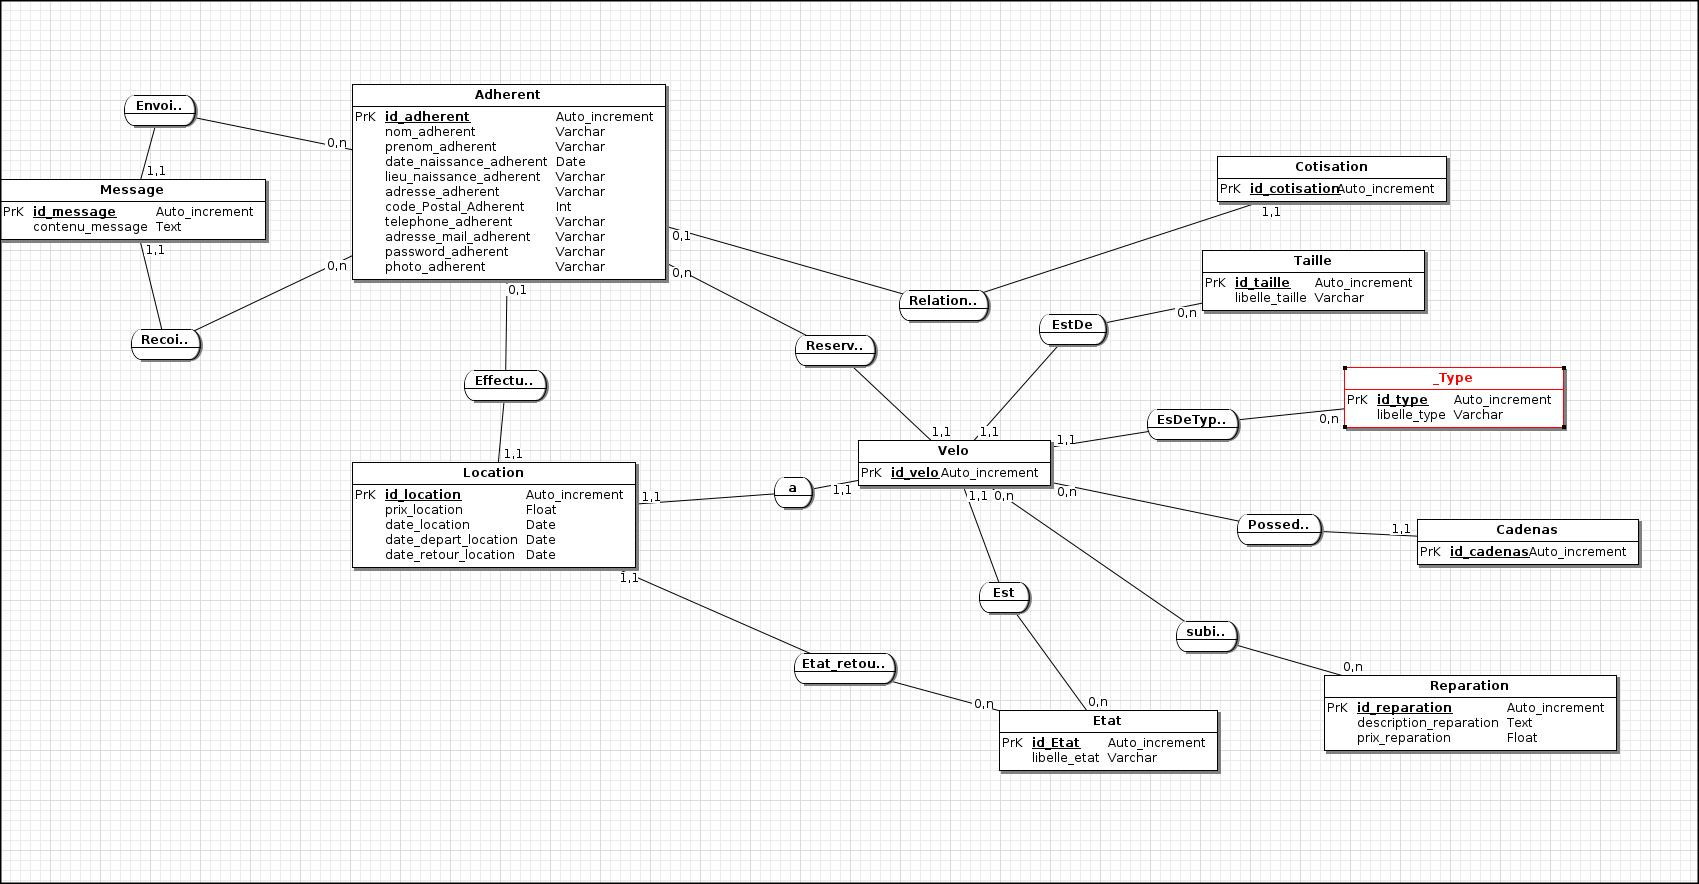
\includegraphics[width=1\textwidth]{MCD.jpg}~
\end{center}

\section{La réalisation du MCD}

\chapter{Le fonctionnement du site Internet}

\chapter{Les problèmes rencontrés}

\chapter{Les améliorations possibles}

\chapter*{Conclusion}
\end{document}



